\section{Competitive Insurance Pricing Market}
\subsection{Model selection}
Our initial work used the optimal model found in Part 2 (adapted for additional features). However, we found that, because the dataset for part 3 has more features than part 2, our model was not optimal and a more complex model performed better (our model architectures for the non-linear and linear models are outlined in \autoref{fig:modelarchitectures}). We optimised our model to maximise the area under the AUC-ROC curve, and we found that by increasing the complexity of the model it was better able to identify low risk customers who were unlikely to make a claim (i.e. precision on class 0). This was consistent with our pricing startegy, as discussed below. As in part 2, we employed SMOTE to address class imbalance issues.

Additionally, whilst retaining the sample preprocessing pipeline used in Part 2, we chose to use the \texttt{RobustScaler} from scikit-learn in place of the \texttt{StandardScaler} owing to the existence of more anomolous datapoints in some of the features introduced in Part 3.
\subsection{Calibration}
Both models were calibrated using the scikit-learn \texttt{CalibratedClassifier class}, requiring the use of the keras \texttt{KerasClassifier} wrapper and our own wrapper class to match the method provided. The corresponding ROC curves are shown in
\autoref{fig:calibroc}, which shows that the calibration of probabilities outputted by our classifier made little difference to the ROC curves. However, calibration had a positive impact on our performance in the AI market; with uncalibrated probabilities, there is no consistent connection between the model output and the risk factor of an individual. It simply states that if person A is has a higher model output than person B, A is riskier than B, but with no quantifiable measure of "how much riskier". The calibrated model outputs correspond more closely to a frequency model, therefore it is no surprise that the calibrated model performs better in the AI insurance market.

\begin{figure}[h!]
    \centering
    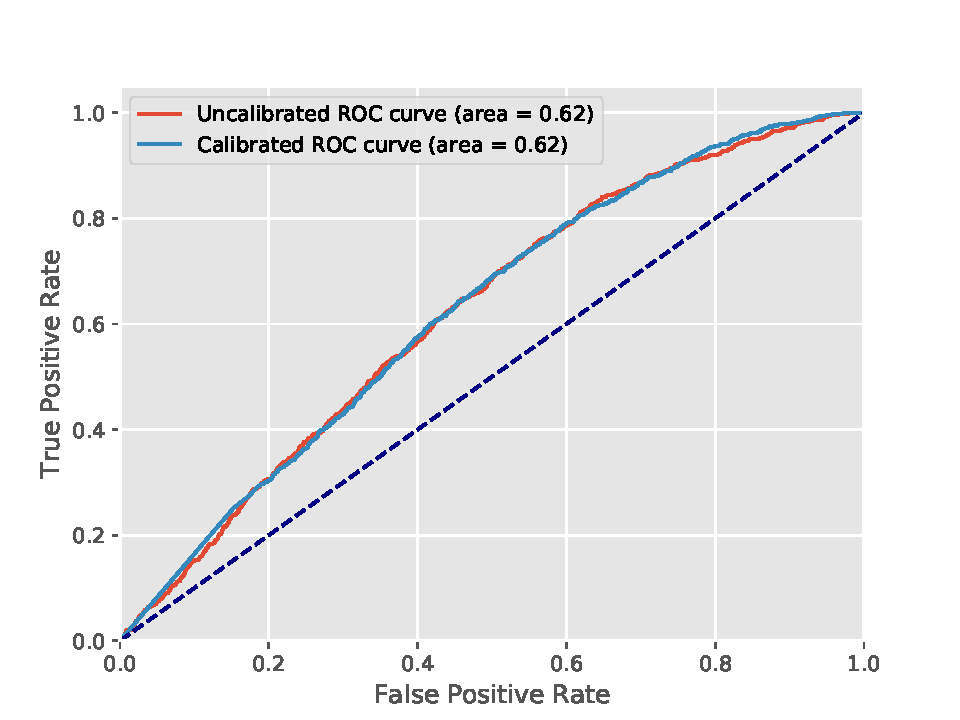
\includegraphics[width=0.6\textwidth]{figures/calibrationROC.pdf}
    \caption[Part 3: ROC curves showing the effect of calibration]{ROC curves showing the effect of calibrating the non-linear classifier.}
    \label{fig:calibroc}
\end{figure}

\subsection{Pricing Strategy}

Our pricing strategy was to identity and win contracts for the low risk customers. Our hypothesis was that by winning these customers' contracts we could minimize our claim-per-customer, and therefore could translate much of the revenue from selling contracts into profit. The price offered was the product of the frequency model (our calibrated base classifier) and the severity model (which was just the mean claim as written in the skeleton code) plus a margin. By setting a relatively high margin we were able to make good profits on the low risk customers and made us too expensive for the high risk customers so we did not win their contracts.

The successful execution of our strategy manifests through the performance of our insurance pricing agent. The mean price won was the lowest in the market (£44) (as we were aiming for the low-risk customers therefore had to offer cheap premiums to win them) and the mean loss incurred was also the lowest in the market at £35 (excluding agents that did not receive any claims). Additionally, our mean price offered was the highest in the market at £153. These imply all three of the pillars of our pricing strategy were successfully executed as we won the contracts of low risk customers, hence did not receive large claims and also did not win the contracts of high risk customers. This is how we managed to achieve a 3rd place ranking in the AI market.

\subsection{Linear Model Comparison}
\label{sec:linmodel}
Our linear model used a logisitic regression classifier (implemented as a one-layer neural network with sigmoid activation function utilising our existing code base (i.e. a single-layer perceptron)). Our linear model also performed well, making around half of the profit of our non-linear agent. 

The base classifier in the linear model performs similarly well to our non-linear base classifier. The PCA analysis in \autoref{section:explor} offers some insight as to why this is (as the part 2 data is a subset of part 3 data the results from running PCA on part 3 data do not differ significantly to the part 2 data). As noted in the earlier discussion of \atoref{fig:pca} in which we performed PCA the dataset, we have observed that the linear combinations of features account for the majority of correlation between labels and sets of features. As such, it is not surprising that the linear model performs relatively well. Indeed, we observed that many "semi-complex" network architectures actually performed worse than the single-layer perceptron, as their additional complexity was insufficient to capture any more nuanced and obscure trends in the data, whilst also hampering their ability to concisely represent the linear behaviour which predominantly determines the correlation in the data. 

To make matters worse, this means that we are faced with an optimization problem in which improving beyond the linear model requires a complicated network, which when coupled with the relatively small amount of data and dominance of the linear correlations makes it very difficult to converge on a superior optimum. This was indeed what we observed during the training and tuning of our final network architecture.

\newpage

\subsection{LabTS Complications}
We faced numerous substantial difficulties getting our implementations (for part 2 as well as part 3) to pass the LabTS tests. One such difficulty was converting categorical features to dummies so they could be used in the network. However, these ran into difficulties with LabTS and so (after spending a substantial amount of time identifying the issue) we decided to discard all categorical features. This harmed the performance of our model as it meant we discarded many useful features. This was one of the many complications we faced with LabTS, and cumulatively these took a substantial amount of time to overcome.

Our code never passed the tests on LabTS. However, it did pass the tests when we downloaded them and we gather from Piazza that this means our models should pass the tests upon assessment.

